%%%%%%%%%%%%%%%%%%%%%%%%%%%%%%%%%%%%%%%%%%%%%%%%%%%%%%%%%%%%%%%%%%%%%%
% Date:
%     19.10.2018
%
% Course:
%     SEN - Intelligent Sensors
%     https://www.fit.vutbr.cz/study/courses/index.php.en?id=12918
%
% Project:
%     Commissioning Heartbeat Sensor and Comparison Against Oximeter
%
% Authors:
%     Adrián Tóth, xtotha01@stud.fit.vutbr.cz
%     Jiří Záleský, xzales12@stud.fit.vutbr.cz
%%%%%%%%%%%%%%%%%%%%%%%%%%%%%%%%%%%%%%%%%%%%%%%%%%%%%%%%%%%%%%%%%%%%%%

\documentclass[11pt,a4paper]{article}

\usepackage[left=2cm,text={17cm,24cm},top=3cm]{geometry}
\usepackage[english]{babel}
\usepackage[utf8]{inputenc}
\usepackage[T1]{fontenc}

\usepackage{url}
\usepackage{float}
\usepackage{xcolor}
\usepackage{siunitx}
\usepackage{listings}
\usepackage{hyperref}
\usepackage{textcomp}
\usepackage{breakurl}
\usepackage{etoolbox}
\usepackage{graphicx}
\usepackage{supertabular}
\usepackage{indentfirst}
\usepackage[titles]{tocloft}

\renewcommand{\cftdot}{}

\def\UrlBreaks{\do\/\do-}
\newcommand{\tilda}{\raisebox{0.5ex}{\texttildelow}}

\graphicspath{{.}}
\patchcmd{\thebibliography}{\section*{\refname}}{}{}{}
\definecolor{stringcolor}{RGB}{178, 163, 19}

\lstset{
    frame=tb,
    tabsize=2,
    numbers=left,
    framexleftmargin=25pt,
    xleftmargin=.141\textwidth,
    linewidth=40em,
    breaklines=true,
    basicstyle=\scriptsize\ttfamily,
    commentstyle=\color{gray},
    keywordstyle=\color{red},
    stringstyle=\color{stringcolor},
    otherkeywords={>,<,*,&,|,+,-,!,=,~},
    emph={int,char,double,float,unsigned},
    emphstyle={\color{blue}}
}


% #################################################################################################
\begin{document}
% #################################################################################################


% #################################################################################################
% TITLEPAGE
\begin{titlepage}
    \begin{center}
        \Huge
        \textsc{
            Faculty of Information Technology\\
            Brno University of Technology
        }
        \vspace{80px}
        \begin{figure}[!h]
            \centering
            
\includegraphics[scale=0.3]{img/vutbr-fit-logo.eps}
        \end{figure}
        \\[15mm]
        \Huge{
            \textbf{
                SEN
            }
        }
        \\[1.5mm]
        \huge{
            \textbf{
                Intelligent Sensors
            }
        }
        \\[2.5em]
        \LARGE{
            \textbf{
                Commissioning Heartbeat Sensor and Comparison\\
                Against Oximeter
            }
        }
        \vfill
    \end{center}
        \Large{
            \hfill\\
            Jiří Záleský (xzales12)\\
            Adrián Tóth (xtotha01)\hfill \today
        }

\end{titlepage}


% #################################################################################################
% CONTENT


\setlength{\parskip}{0pt}
\hypersetup{hidelinks}\tableofcontents
\setlength{\parskip}{0pt}

\newpage

\section{Project}

The aim of this project is to comission a heart beat sensor. Within the project, there will be done several measurements, which will be later compared with the results of a valid device - oximeter. Prof. Ing., Dipl.-Ing. Martin Drahanský, Ph.D\footnote{\href{http://www.fit.vutbr.cz/~drahan/}{www.fit.vutbr.cz/{\tilda}drahan}} is the project supervisor.

\section{Abstract}

The aim of this project is to demonstrate a method of measuring heart beat via infrared light. The upcoming sections will describe further requirements to achieve the right functionality. The results of measurement were compared with a valid heart beat sensor, which measured heart beat in the same way as the infrared method. The reference device is sufficiently improved to ensure that the measurements are accurate enough, to consider them as valid.

\section{Introduction}\label{sec:intro}

The infrared light has a key role in this project. The infrared LED represents a main source of infrared rays which are sent in a direction to phototransistor. These rays may be affected by any kind of object representing a blockade in the way to the phototransistor. Using a finger as a rays blockade, the rays are affected not only by the finger itself, but also by the blood in the finger. As the heart is pulsing inside of the person's body, the blood pressure is different inside of the finger's veins, which has also a great impact on the rays. The emitted rays from the finger are detected by the phototransistor that produces a precise values. Based on these values, there is a possibility to detect heart beat. This method of measurement is shown in Figure \ref{fig:method}.

\begin{figure}[H]
    \centering
    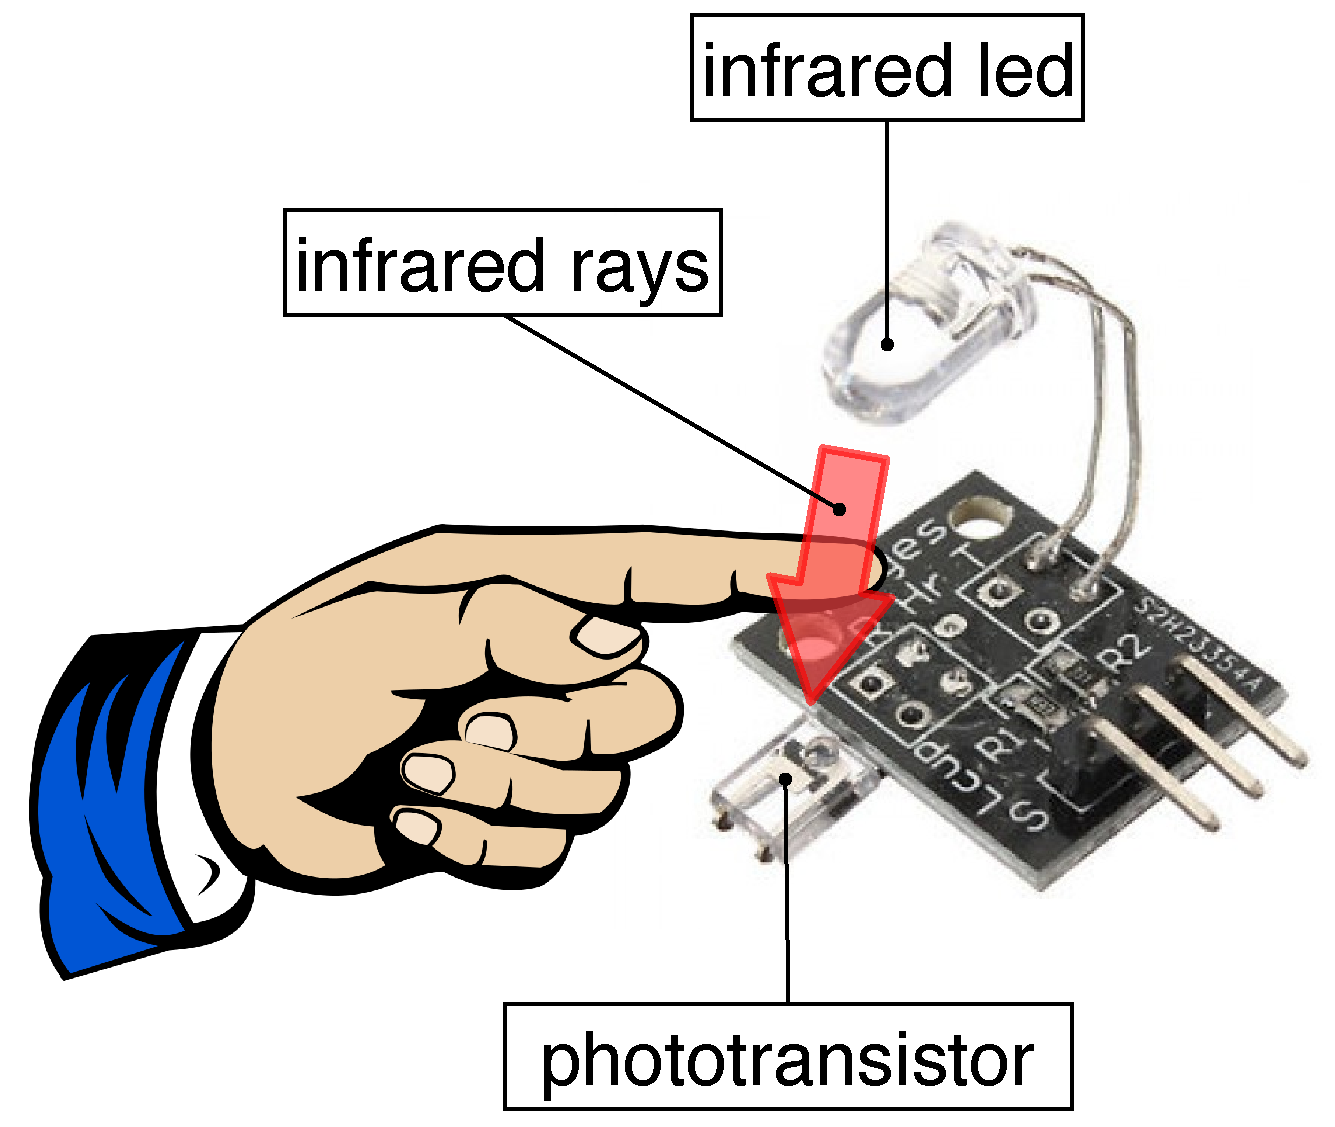
\includegraphics[scale=0.4]{img/infrared_method.pdf}
    \caption{Method of infrared heart beat measurement.}
    \label{fig:method}
\end{figure}

\newpage

The necessary facilities for the implementation of the project were:\\[-1.5em]
\begin{itemize}
    \item Device shown in Figure \ref{fig:oldplatform}.\\[-2em]
        \begin{figure}[H]
            \centering
            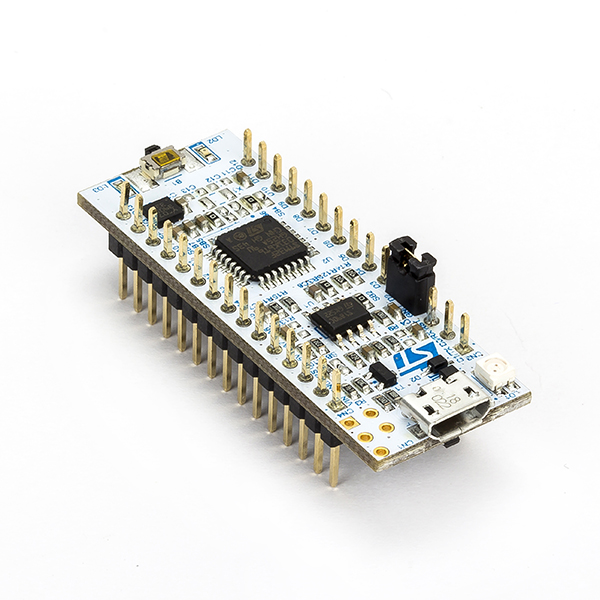
\includegraphics[scale=1.4]{img/device-old.jpg}
            \caption{STM32 Nucleo board~\cite{IMG-DEVICE-OLD}.}
            \label{fig:oldplatform}
        \end{figure}
        \hfill\\[-17mm]
    \item Sensor shown in Figure \ref{fig:senzor1}.
        \begin{figure}[H]
            \centering
            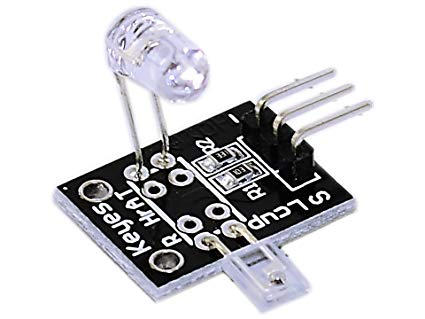
\includegraphics[scale=0.3]{img/sensor1.jpg}
            \caption{Keyes KY-039 Finger Heartbeat Detection Sensor~\cite{IMG-SENSOR-1}.}
            \label{fig:senzor1}
        \end{figure}
        \hfill\\[-18mm]
    \item Three female--to--female jumper wires.\\[-2.5mm]
\end{itemize}

After we received the devices, we faced a lot of problems. The main device representing the basic platform was not working properly so we had to ask for a new one. Later, the main device (shown in Figure \ref{fig:oldplatform}) was replaced to a new one (see Figure \ref{fig:platform1}) due to wrong functionality by the technical assistant of the project - Ing. Tomáš Goldmann\footnote{\href{http://www.fit.vutbr.cz/~igoldmann/}{www.fit.vutbr.cz/{\tilda}igoldmann}}.

\newpage

\begin{figure}[H]
    \centering
    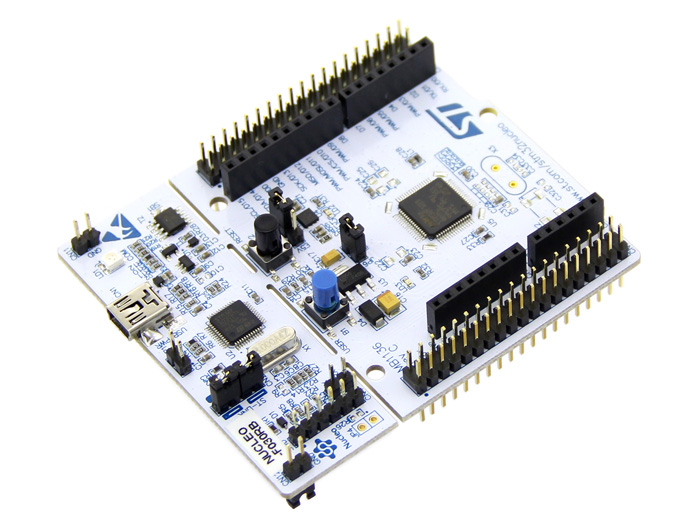
\includegraphics[scale=0.4]{img/device1.jpg}
    \caption{STM32 Nucleo board~\cite{IMG-DEVICE-1}.}
    \label{fig:platform1}
\end{figure}

\indent The device shown in Figure \ref{fig:platform1} - NUCLEO-F030R8~\cite{PLATFORM}, was the main platform for the project. The device was equipped with a STM32F030R8~\cite{MCU} microcontroller unit (MCU), which was designed and made to be suitable for a wide range of applications. MCU includes a set of peripherals through which it communicates with other devices such as the sensor shown in Figure \ref{fig:senzor1}. To create a communication pipeline, these units must be connected to each other via jumper wires. Wires provide a connection between the pins of units and so the pins have to be configured correctly.

\section{Setup}

Firstly, the components must be connected to each other in a right way. Sensor, as a slave component shown in Figure \ref{fig:senzor2wires}, is connected to the main device (master component). These two units are connected via 3 jumper wires to the corresponding pins. The Figure \ref{fig:device2wires} and \ref{fig:senzor2wires} have three common marked pins: \textit{GND} (orange), \textit{5V} (yellow), \textit{PA0} and \textit{S} (green); by which they are connected together. \textit{PA0} indicates an analog input pin to the master component. A precise description of all the necessary pins is shown in Figure \ref{fig:legend}.

\begin{figure}[H]
    \centering
    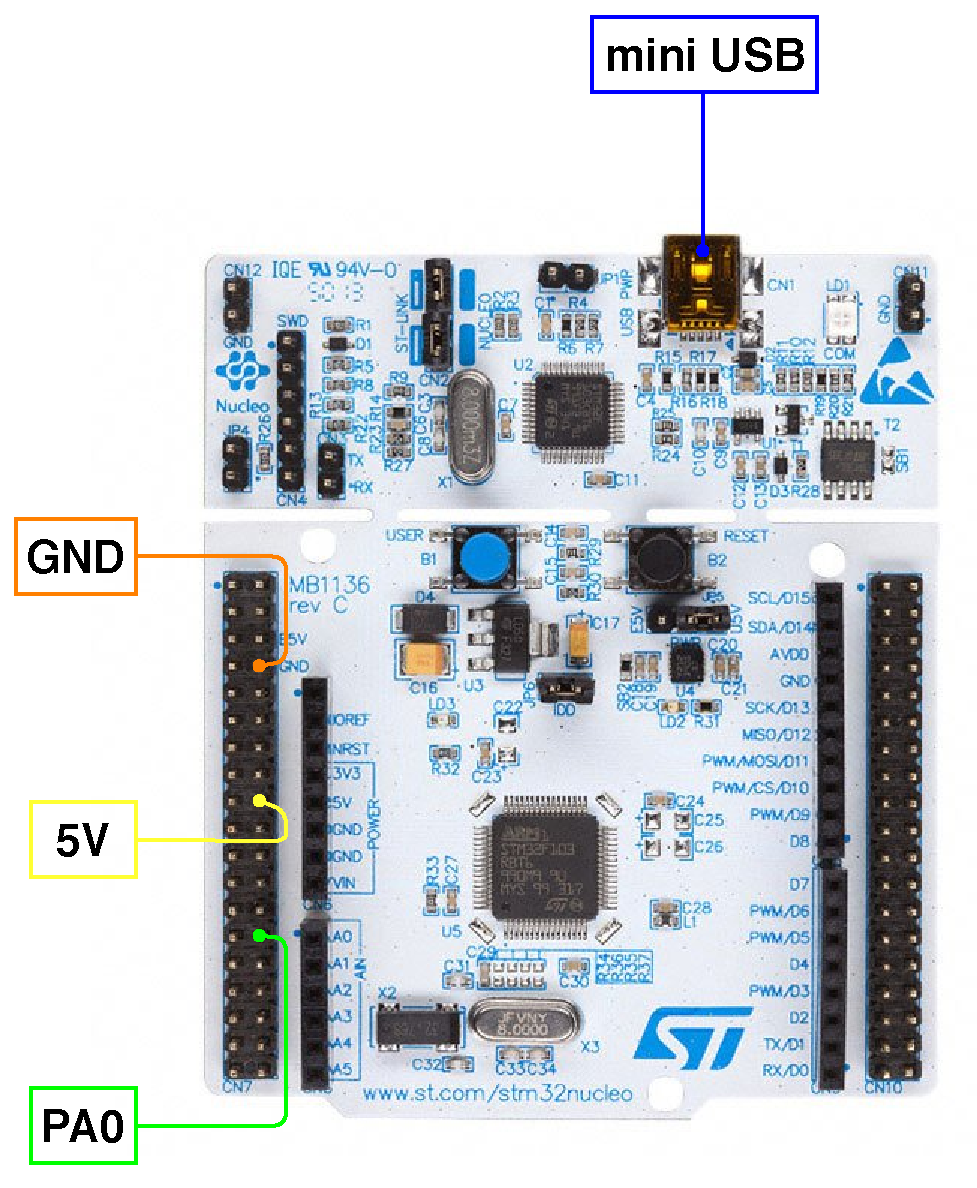
\includegraphics[scale=0.5]{img/device2-wires.pdf}
    \caption{NUCLEO-F030R8~\cite{IMG-DEVICE-2} connection scheme.}
    \label{fig:device2wires}
\end{figure}

\begin{figure}[H]
    \centering
    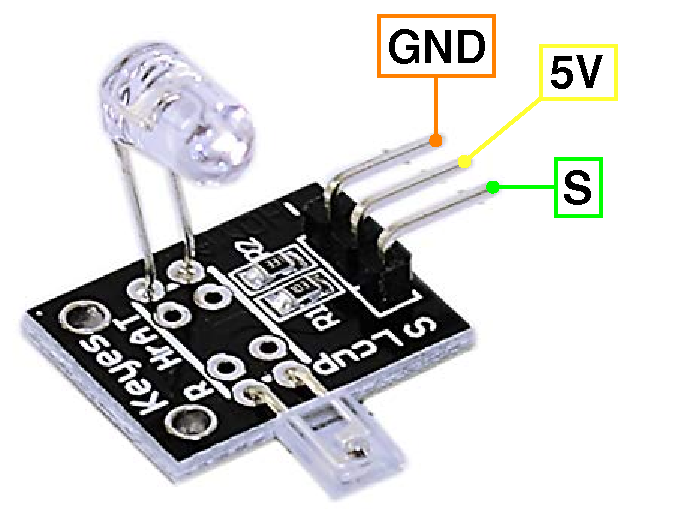
\includegraphics[scale=0.5]{img/sensor1-wires.pdf}
    \caption{Keyes KY-039~\cite{IMG-SENSOR-1} connection scheme relating to Figure \ref{fig:device2wires}.}
    \label{fig:senzor2wires}
\end{figure}

\begin{figure}[H]
    \begin{center}
        \begin{tabular}{|r|l|}
            \hline
            \textbf{S}        & sensor output \\
            \hline
            \textbf{B1}       & button 1 \\
            \hline
            \textbf{B2}       & button 2 \\
            \hline
            \textbf{LD2}      & LED 2 \\
            \hline
            \textbf{GND}      & ground \\
            \hline
            \textbf{5V}       & 5 volt voltage supply \\
            \hline
            \textbf{PA0}      & pin PA0 \\
            \hline
            \textbf{mini USB} & mini USB port \\
            \hline
        \end{tabular}
    \end{center}
    \caption{Explanatory notes.}
    \label{fig:legend}
\end{figure}

A connection scheme of the devices is shown in Figure \ref{fig:old_con_scheme}. After the devices were correctly connected and attached to the computer via mini USB port (see Figure \ref{fig:connection}), they were ready to be programmed.

\begin{figure}[H]
    \centering
    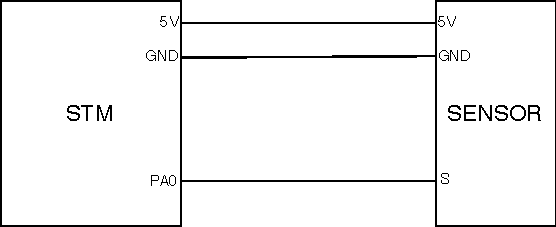
\includegraphics[scale=1.4]{img/old_con_scheme.pdf}
    \caption{Device connection scheme.}
    \label{fig:old_con_scheme}
\end{figure}

\begin{figure}[H]
    \centering
    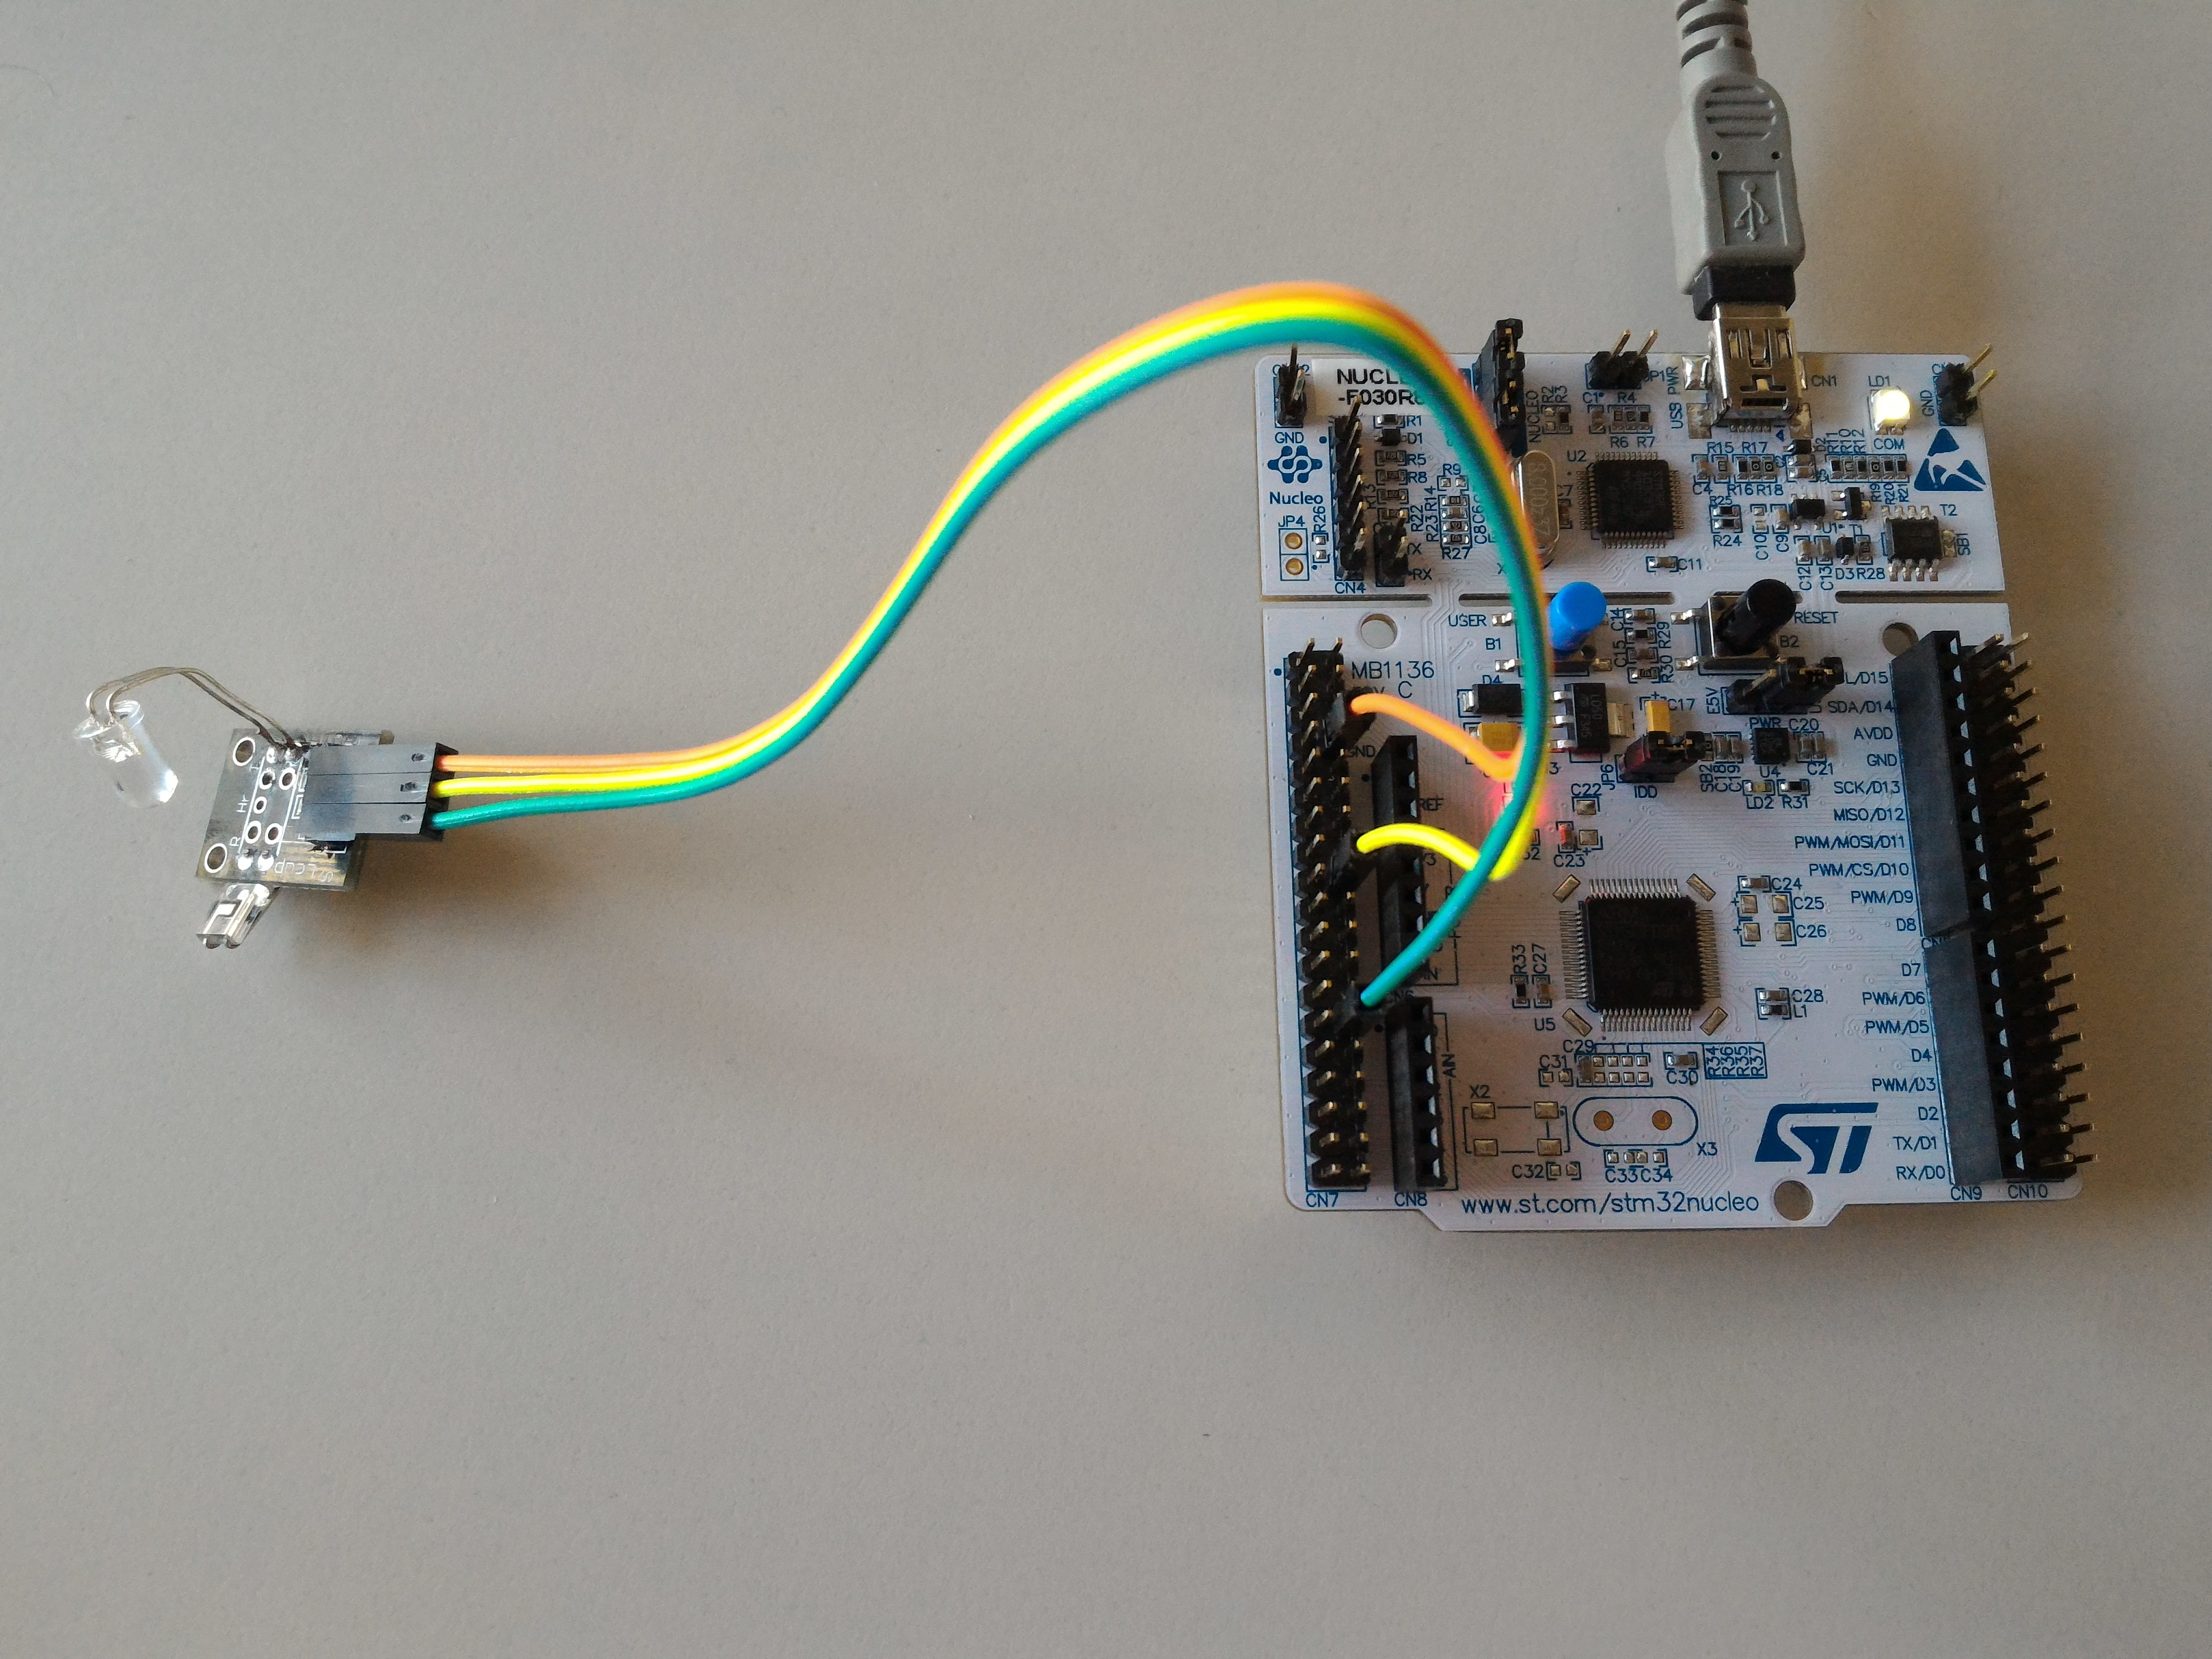
\includegraphics[scale=0.1]{img/setup1.jpg}
    \caption{Correct connection of devices.}
    \label{fig:connection}
\end{figure}

As we were working on the implementation part of the project, there was a measurement anomaly. The results were affected by different input voltage on the pin. We asked for an advice from the technical assistant. He has recommended us a different device connection which is shown in Figure \ref{fig:new_con_scheme}. He suggested to use a protoboard with two 10k\si{\ohm} resistors and a few additional connection wires.

\begin{figure}[H]
    \centering
    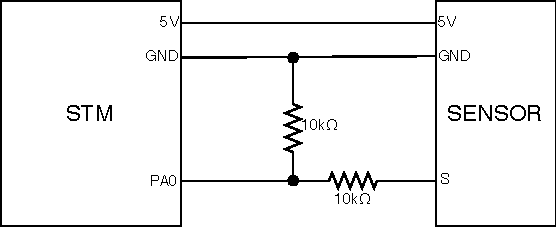
\includegraphics[scale=1.4]{img/new_con_scheme.pdf}
    \caption{New device connection scheme.}
    \label{fig:new_con_scheme}
\end{figure}

The devices have been reconnected based on the given advice, which is shown in Figure \ref{fig:new_dev_con}. This setup was the proper one where the values have not been affected by voltage.

\begin{figure}[H]
    \centering
    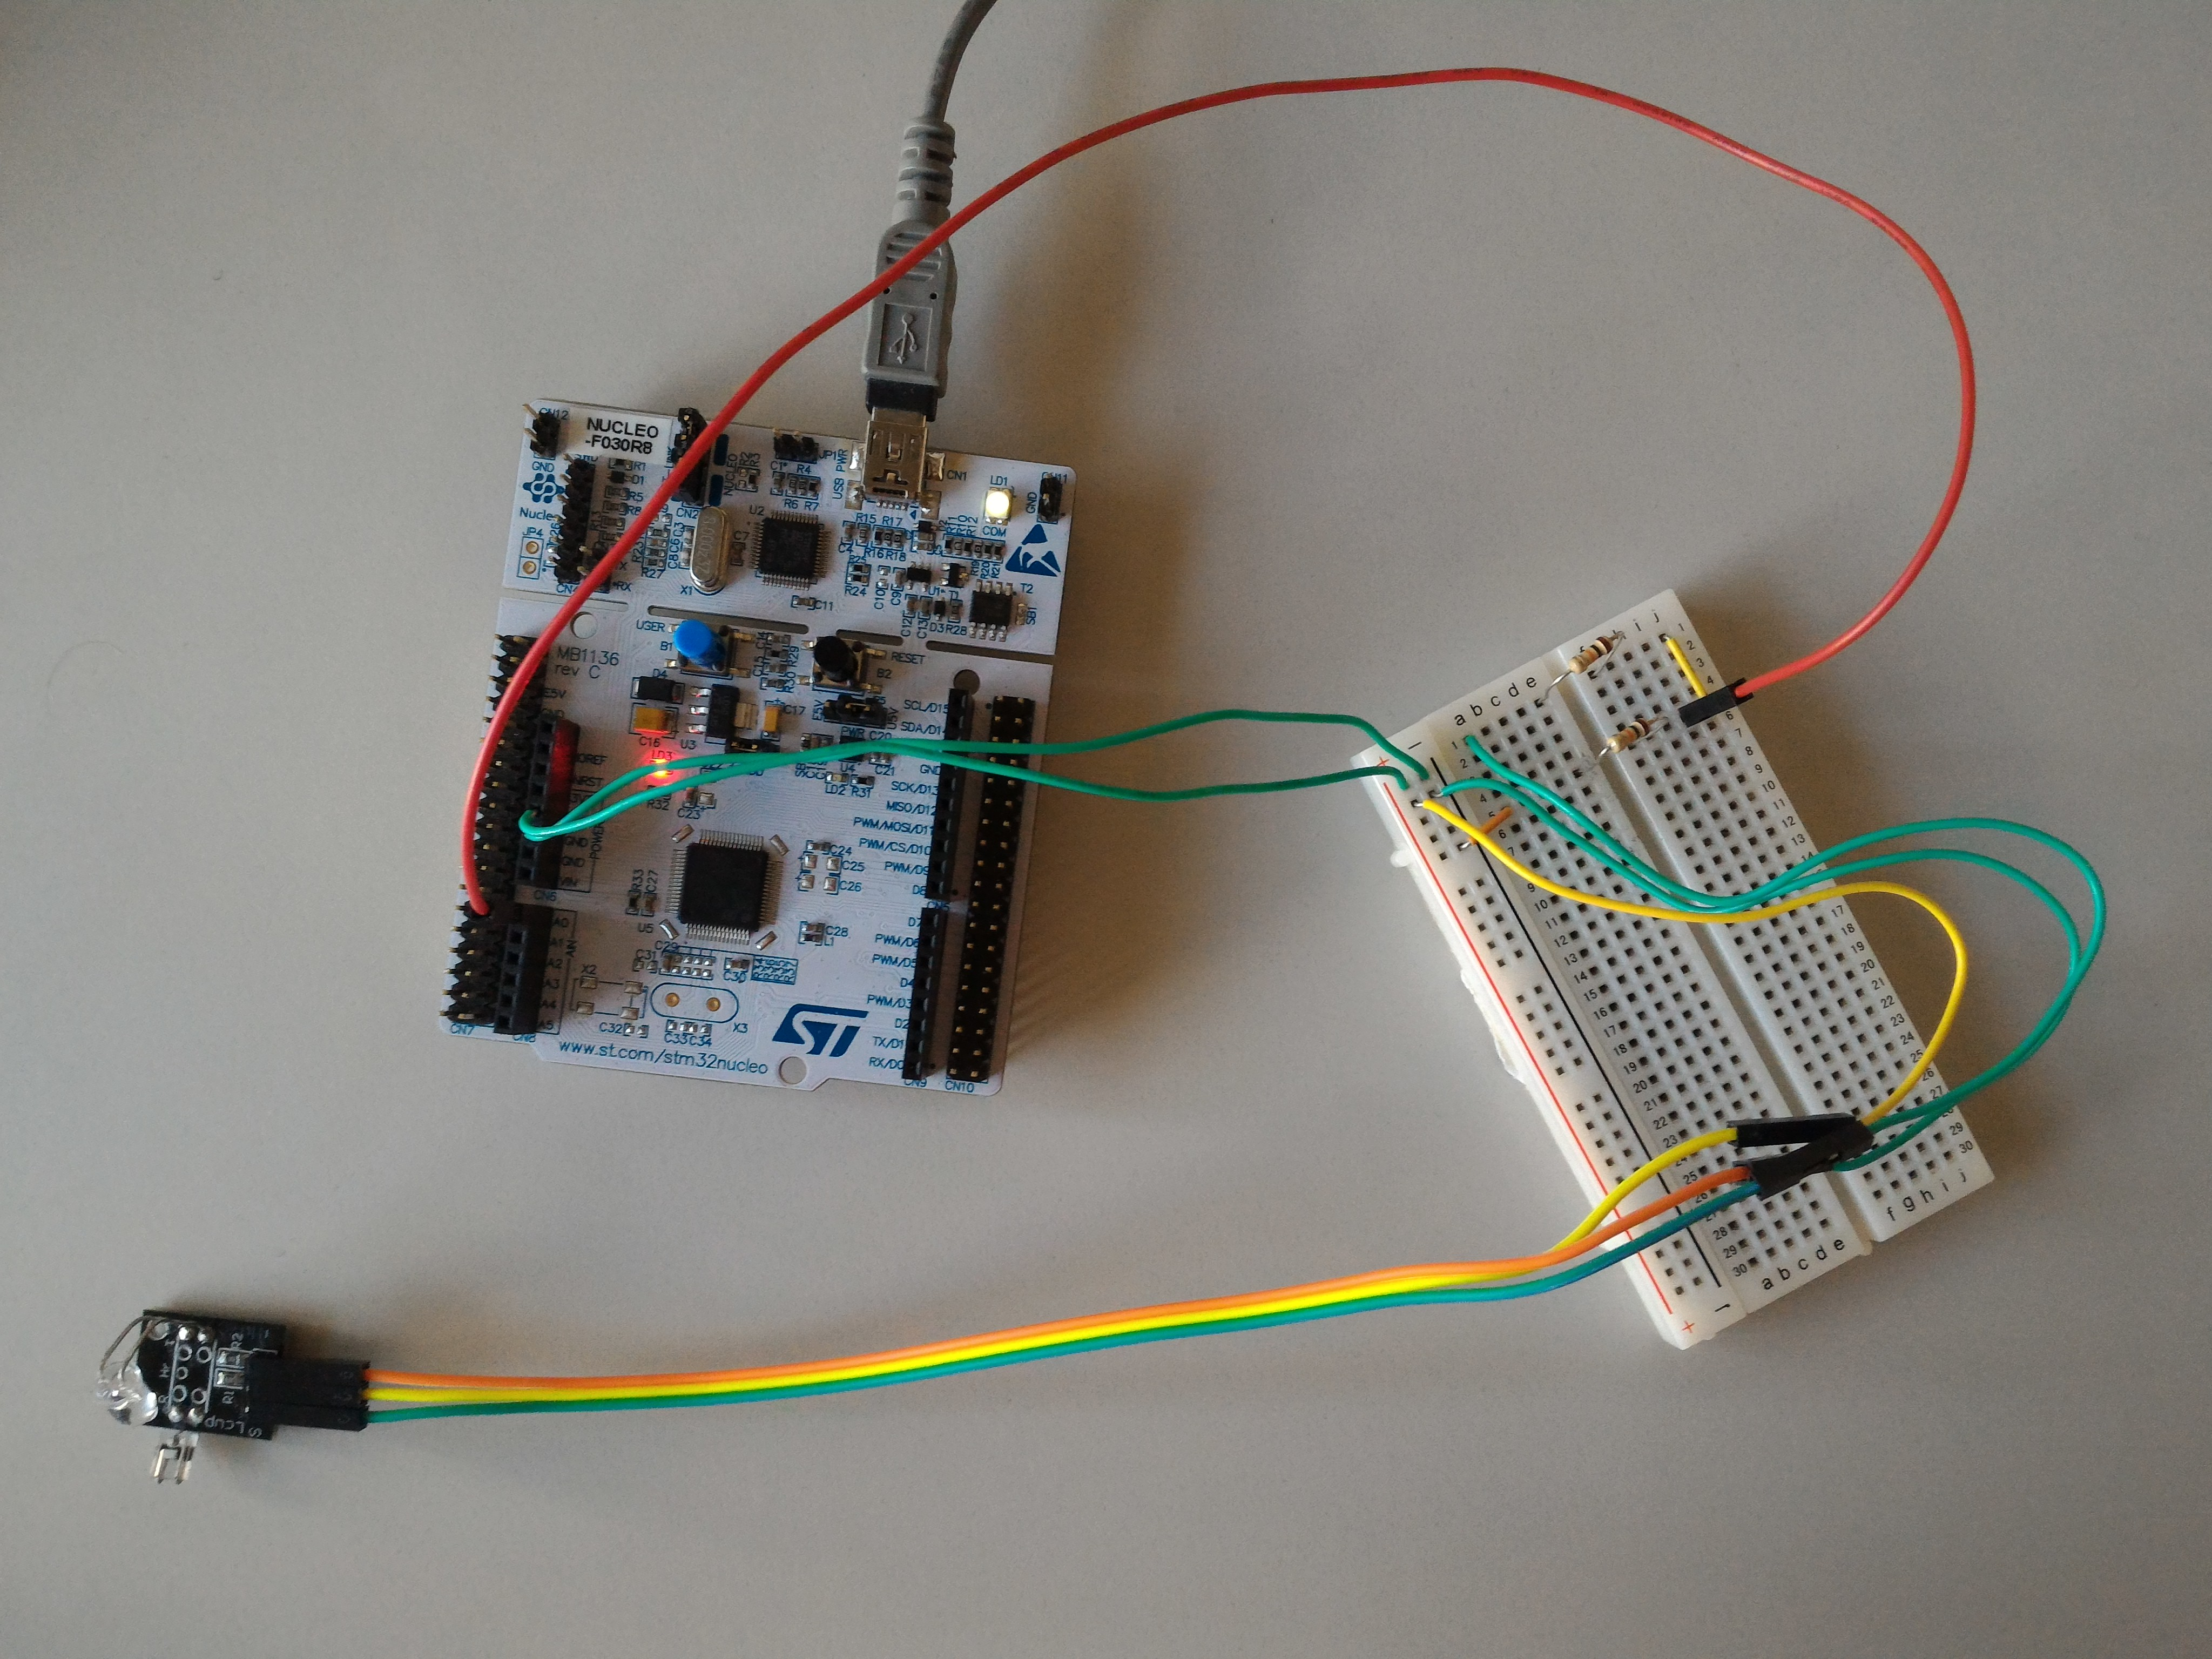
\includegraphics[scale=0.1]{img/setup2.jpg}
    \caption{New connection of devices.}
    \label{fig:new_dev_con}
\end{figure}

\newpage

\section{Implementation}\label{sec:impl}

The implementation is based on an algorithm~\cite{SENSOR}, which detects deviation in a set of incoming values from the sensor. The values, incoming as a sequence of measurements, contain a few that have a certain deviation what indicates the pulse. This is the deviation, which basis we can calculate the hear beat per minutes also know as beats per minute (BPM) on. The program will light up a LED (see LD2 in Figure \ref{fig:device2wires}) on each beat. The BPM is calculated from one period - the time between two hear beats. No history is used for the calculations.\\

We used \textit{Mbed OS 5}\footnote{\href{https://os.mbed.com/}{os.mbed.com}} to develop the necessary code for the right functionality. It is a browser-based IDE, which also includes a build-in compiler. Based on your set device in this IDE, you can compile online and download the binary file. The device may be programmed by writing this binary file to the device directly, which is connected to computer by USB, via any type of file manager. The main source code is shown in Section \ref{subsec:code}.\\

Algorithm itself is a little bit complicated due to dynamic range of incoming values - there is no value from a static interval. The finger position significantly affects the interval of values, but does not have any impact on the deviation between the values. Integers representing the values, are generated between 0 and 65535. The finger position will state a subinterval, which is shifted on that interval based on the finger position due to change of resistance. To detect a deviation, it is necessary to keep a previous value from the sequence. A calculation related to comparing action is provided, which will determine divergence between the values. If this action will establish the deviation as large enough, this value will be determined as a beat at that moment.\\

The precision of the algorithm depends on the device configuration and sensor precision. It is nearly impossible to make a universal algorithm which can determine heart beat on inaccurate values. The more accurate the sensor values, the more precise the results. As an accuracy factor we can count with a finger motion that has the biggest impact on the BPM calculations. By examining the sensor, we can see that the phototransistor is not sealed into rubber. This fact indicates, that the sensor is receiving external infrared rays from the surrounding area. We can assume that the surrounding area can influence the results too.

\section{Mensuration}\label{sec:mensuration}

Measurements were done on fifty different persons with our device and valid device. The values of each measurement are shown in Section \ref{subsec:table}. Each row in a table represents a different person that is numbered. Other columns such as `\textit{Value 1}' contain values measured via sensor, which was presented in Section \ref{sec:intro} -- Introduction. The last column `\textit{Value 2}' includes values measured via valid device - SILVERCREST - Pulsoximeter SPO 55 (see Figure \ref{fig:pulsoximeter1}). Pulsoximeter is simple, smart, compact and easy to use device. The usage is shown in Figure \ref{fig:pulsoximeter2}. Further informations about the correct device usage are shown in video\footnote{\href{https://youtu.be/RMRV1MhwhIw}{youtu.be/RMRV1MhwhIw}}.\\

\newpage

\begin{figure}[H]
    \centering
    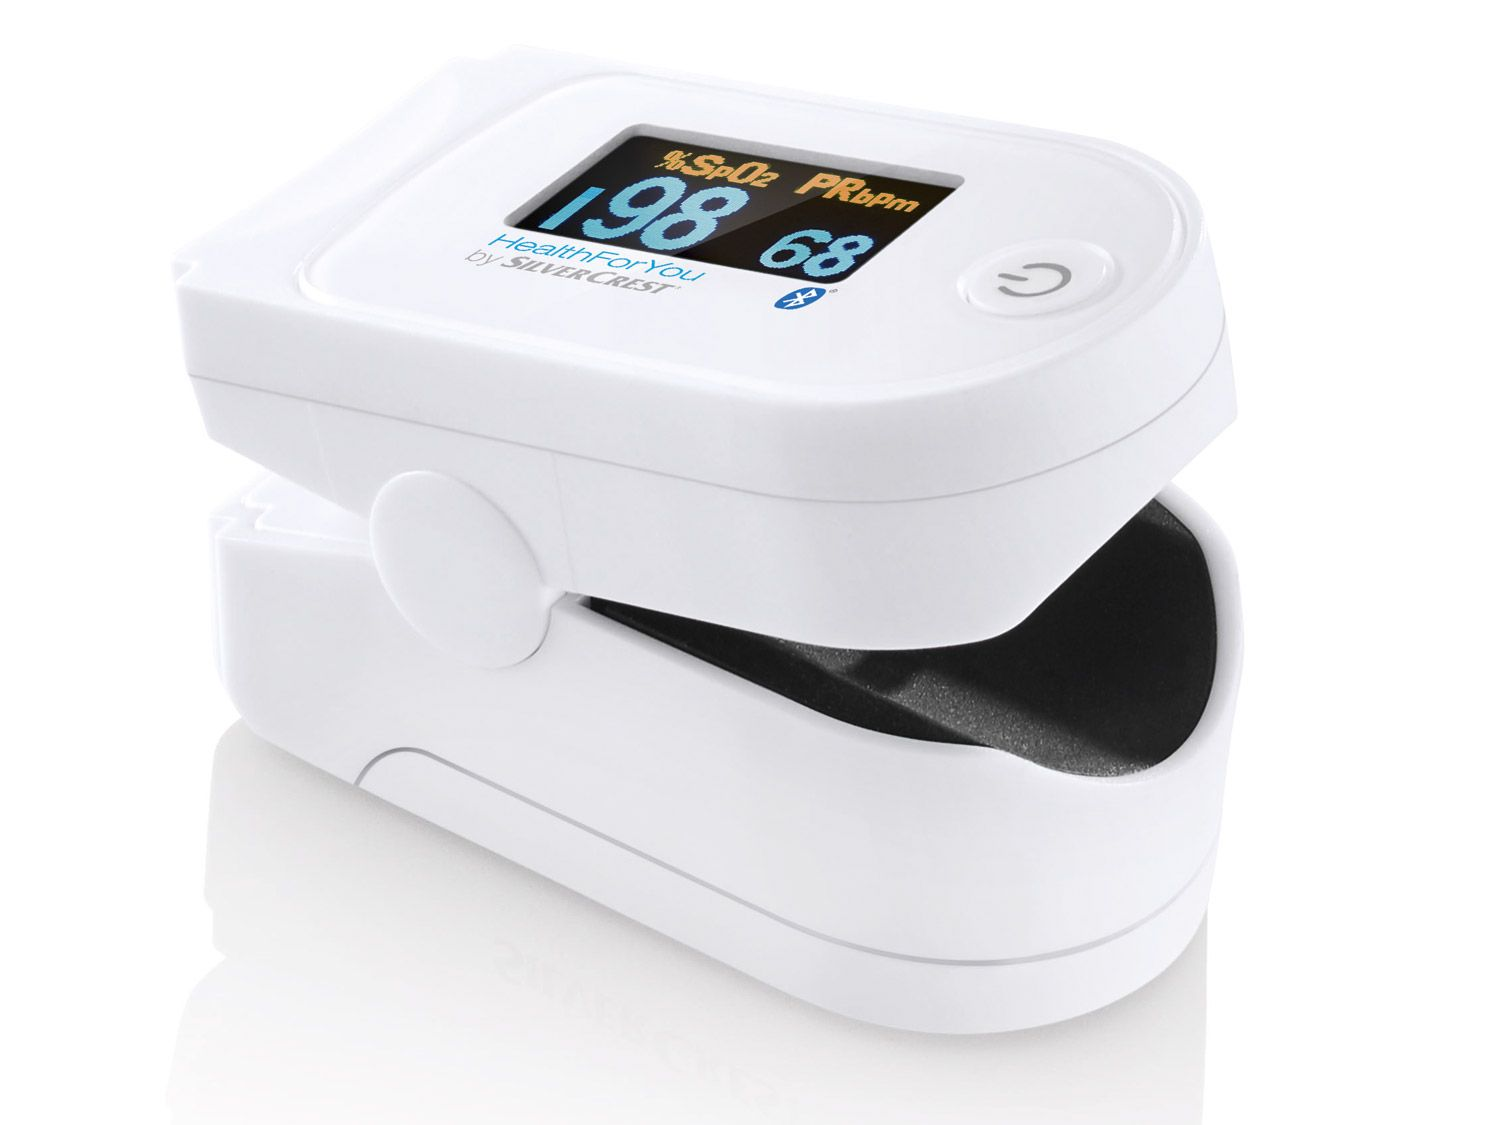
\includegraphics[scale=0.15]{img/pulsoximeter1.jpg}
    \caption{SILVERCREST - Pulsoximeter SPO 55~\cite{IMG-PULSOXIMETER-1}.}
    \label{fig:pulsoximeter1}
\end{figure}

\begin{figure}[H]
    \centering
    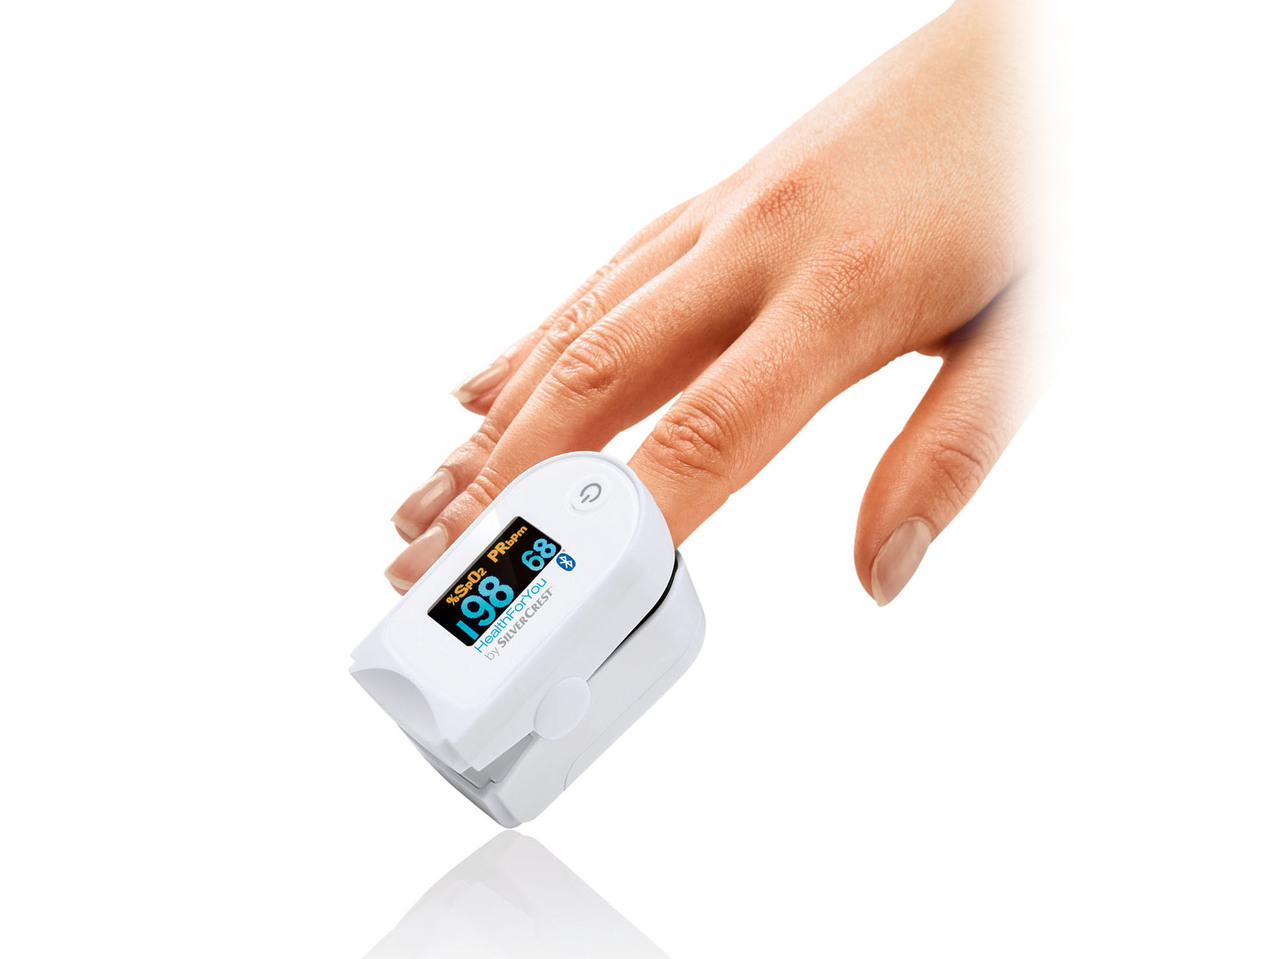
\includegraphics[scale=0.7]{img/pulsoximeter2.jpg}
    \caption{Usage of pulsoximeter~\cite{IMG-PULSOXIMETER-2}.}
    \label{fig:pulsoximeter2}
\end{figure}

Based on the measurements, we can calculate statistical values on which basis we can determine the precision of our implementation. The calculated statistical values are shown in Table \ref{tab:stats}.\\

\begin{table}[H]
  \begin{center}
    \begin{tabular}{r|l}
      average absolute error & 6,08\\
      average relative error & 8,44\%\\
      the greatest deviation & 40,00\%\\
      the smallest deviation & 0,00\%\\
    \end{tabular}
    \caption{Statistical values.}
    \label{tab:stats}
  \end{center}
\end{table}

As we can see the deviations in Table \ref{tab:stats}, some of the measurements are equal to reference device, but some of them are not sufficiently accurate to be considered as valid. As we were testing our device, we have detected that these differences may be reduced by meeting following conditions: the finger is in a correct position, the area has no impact on the phototransistor, the person is not under stress or any kind of effect, that invalidate the mensuration excluding heart diseases (e.g. heart arrhythmia), which has to be detected.

\section{Conclusion}
Based on experiments, calculations and measurements we can state the following judgment. Our device is not enough precise to measure hear beat, but the method of heart beat detection via infrared light can work with better enhanced devices and more precise sensor. There are many influencing factors that devalued the results. Factors may be caused by the area itself but also, the major ones, are cause by the inaccuracy of the sensor. The inaccuracies are described in Section number \ref{sec:impl} and \ref{sec:mensuration}.\\

We have done a few measurements on people with heart arrhythmia, but we could not detect that irregular behaviour of the hear beat. Our device is not capable to detect these irregularities due to inaccuracies.

\newpage

\section{Appendix}
\subsection{Table of measurements}\label{subsec:table}
\vspace*{0,7cm}
\begin{center}
    \tablehead{\hline\textbf{Person} & \textbf{Value 1} & \textbf{Value 2}\\\hline}
    \begin{supertabular}{|c|c|c|}
        1 & 85 & 79 \\\hline
        2 & 95 & 94 \\\hline
        3 & 88 & 70 \\\hline
        4 & 77 & 89 \\\hline
        5 & 86 & 83 \\\hline
        6 & 72 & 67 \\\hline
        7 & 86 & 96 \\\hline
        8 & 74 & 62 \\\hline
        9 & 80 & 83 \\\hline
        10 & 85 & 64 \\\hline
        11 & 64 & 60 \\\hline
        12 & 84 & 60 \\\hline
        13 & 60 & 66 \\\hline
        14 & 57 & 59 \\\hline
        15 & 83 & 81 \\\hline
        16 & 75 & 61 \\\hline
        17 & 76 & 65 \\\hline
        18 & 89 & 80 \\\hline
        19 & 61 & 72 \\\hline
        20 & 63 & 74 \\\hline
        21 & 74 & 58 \\\hline
        22 & 69 & 75 \\\hline
        23 & 67 & 68 \\\hline
        24 & 92 & 99 \\\hline
        25 & 120 & 119 \\\hline
        \end{supertabular}
        \begin{supertabular}{|c|c|c|}
        26 & 64 & 65 \\\hline
        27 & 67 & 66 \\\hline
        28 & 72 & 65 \\\hline
        29 & 92 & 95 \\\hline
        30 & 66 & 64 \\\hline
        31 & 60 & 62 \\\hline
        32 & 73 & 74 \\\hline
        33 & 65 & 68 \\\hline
        34 & 65 & 66 \\\hline
        35 & 105 & 106 \\\hline
        36 & 72 & 81 \\\hline
        37 & 68 & 71 \\\hline
        38 & 91 & 88 \\\hline
        39 & 61 & 63 \\\hline
        40 & 67 & 66 \\\hline
        41 & 115 & 112 \\\hline
        42 & 95 & 79 \\\hline
        43 & 90 & 99 \\\hline
        44 & 73 & 69 \\\hline
        45 & 75 & 75 \\\hline
        46 & 96 & 92 \\\hline
        47 & 89 & 87 \\\hline
        48 & 90 & 88 \\\hline
        49 & 86 & 89 \\\hline
        50 & 122 & 127\\\hline
    \end{supertabular}
\end{center}

\newpage
\subsection{Source code}
\label{subsec:code}

\vspace{0,5cm}
\begin{lstlisting}[language=C++, basicstyle=\tiny, frame=single]
#include "mbed.h"

AnalogIn analog_value(A0);
DigitalOut led(LED1);
int delayTime = 10;

#define LED_ON { led = 1; }
#define LED_OFF { led = 0; }

bool measurement() {
    static int maxValue = 0;
    static bool spikeDetected = false;
    int analogValue;
    bool result = false;

    // analogValue from 0 to 65535
    analogValue = analog_value.read_u16();

    // Voltage measurement transformation
    analogValue = analogValue >> 6; // DIV 64 -> change to 0 - 1023
    analogValue *= (1000 / delayTime);

    // The last maxValue will be detected as a peak.
    if (analogValue * 4L < maxValue) {
        maxValue = analogValue * 0.8;
    }

    // Beat detection
    if (analogValue > maxValue - (1000 / delayTime)) {

        // Change maximum value for next measurement
        if (analogValue > maxValue) {
            maxValue = analogValue;
        }

        // Allocate only one heartbeat to a peak.
        if (spikeDetected == false) {
            result = true;
        }

        spikeDetected = true;
    }
    else if (analogValue < maxValue - (3000 / delayTime)) {
        spikeDetected = false;

        // Change maximum value for remove fake beats
        maxValue -= (1000 / delayTime);
    }

    return result;
}

int main() {
    int beatFrequency;
    int beatsPerMin = 0;

    while(1) {
        if (measurement()) {
            LED_ON;

            // Count beats per minute
            beatFrequency = 60000 / beatsPerMin;

            if (beatFrequency > 50 & beatFrequency < 200) {
              printf("Heart beat frequency: %d BPM\r\n", beatFrequency);
            }

            beatsPerMin = 0;
        }
        else {
            LED_OFF;
        }

        wait_ms(delayTime);
        beatsPerMin += delayTime;
    }
}
\end{lstlisting}

\newpage %#########################################################################################

\section{References}
\bibliographystyle{englishiso}
\begin{flushleft}
    \bibliography{quotation}
\end{flushleft}


% #################################################################################################
\end{document}
% #################################################################################################